\chapter{Diseño}
\label{cap:capitulo4}

En este capítulo se describe el trabajo realizado y los experimentos llevados a cabo para validar el desarrollo.\\

El trabajo, como se explicó en el capítulo 2, se ha dividio en dos fases; primero se realiza una simulación del coche autónomo en una ciudad simplificada, para a continuación, reproducir ese mismo escenario en un entorno real.\\

\section{Entorno simulado}
Para poder simular el comportamiento deseado en un entorno simulado es necesario disponer de dos elementos; un modelo del coche autónomo y un mundo dinámico con el que el vehículo interactuará, todo ello ejecutado dentro de un simulador, en este caso, como se explicó anteriormente, en \textit{Gazebo}.\\

\subsection{Modelo de la ciudad}
Existen numerosos mundos diseñados para Gazebo disponibles en repositiorios de GitHub\footnote{\url{https://github.com/chaolmu/gazebo_models_worlds_collection}}\footnote{\url{https://github.com/mlherd/Dataset-of-Gazebo-Worlds-Models-and-Maps}}. En el caso que se plantea, es necesario una ciudad, por lo que partiendo de una ciudad\footnote{\url{https://github.com/chaolmu/gazebo_models_worlds_collection/blob/master/worlds/small_city.world}} de gran tamaño se reduce su tamaño con el objetivo de, posteriormente, poder reproducir ese escenario en el mundo real. En la figura \ref{fig:city} se observan ambas ciudades.\\

\begin{figure} [h!]
	\begin{center}
		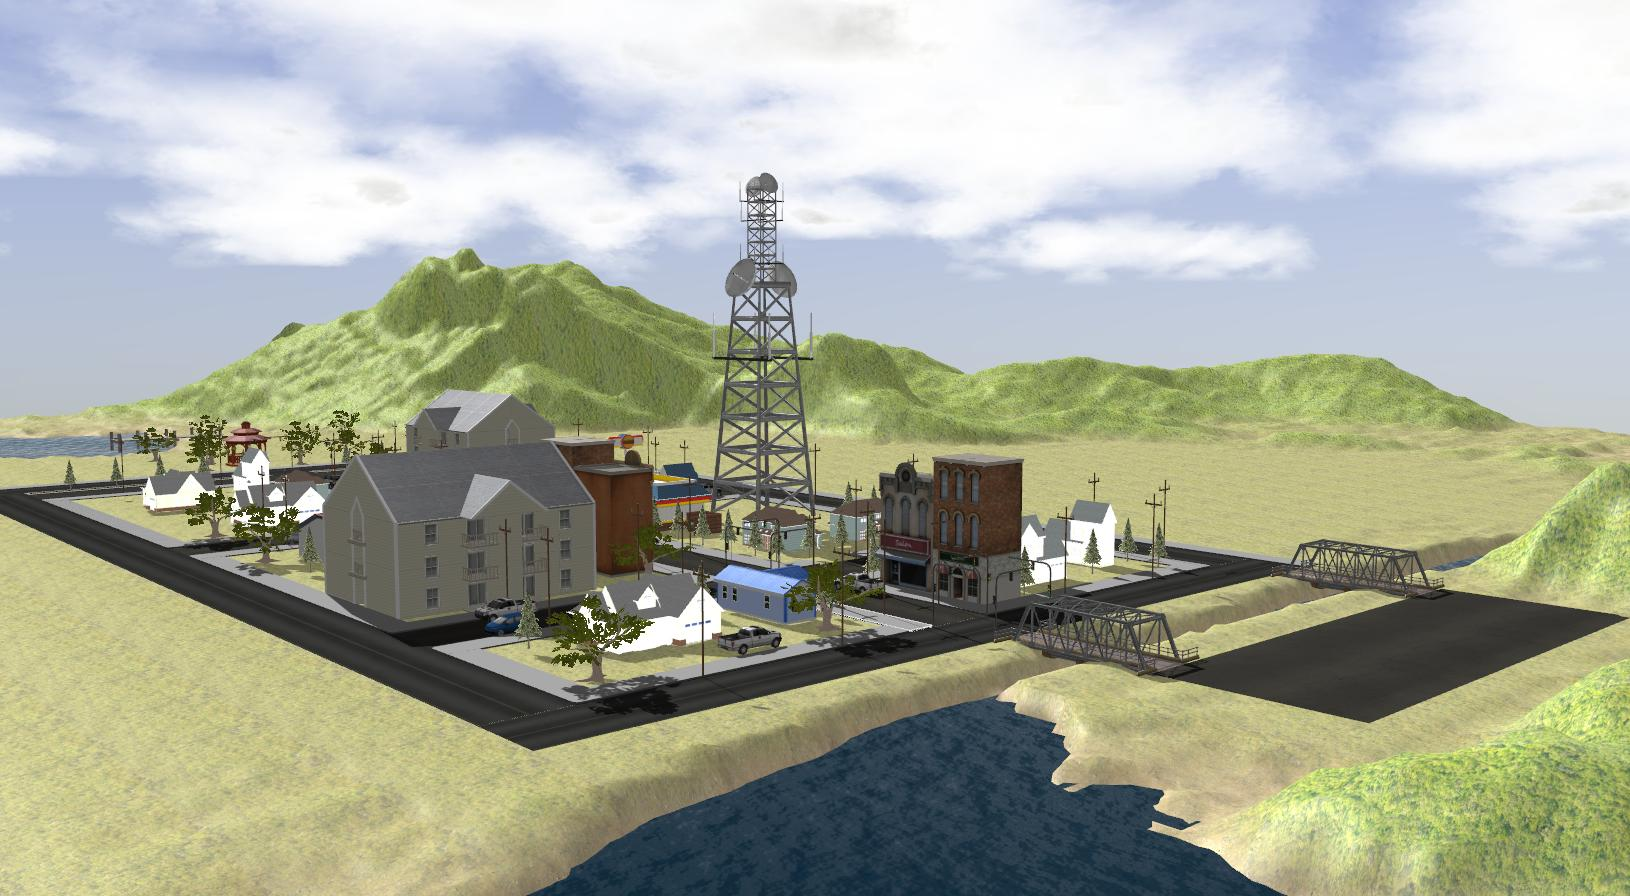
\includegraphics[width=8cm]{figs/city}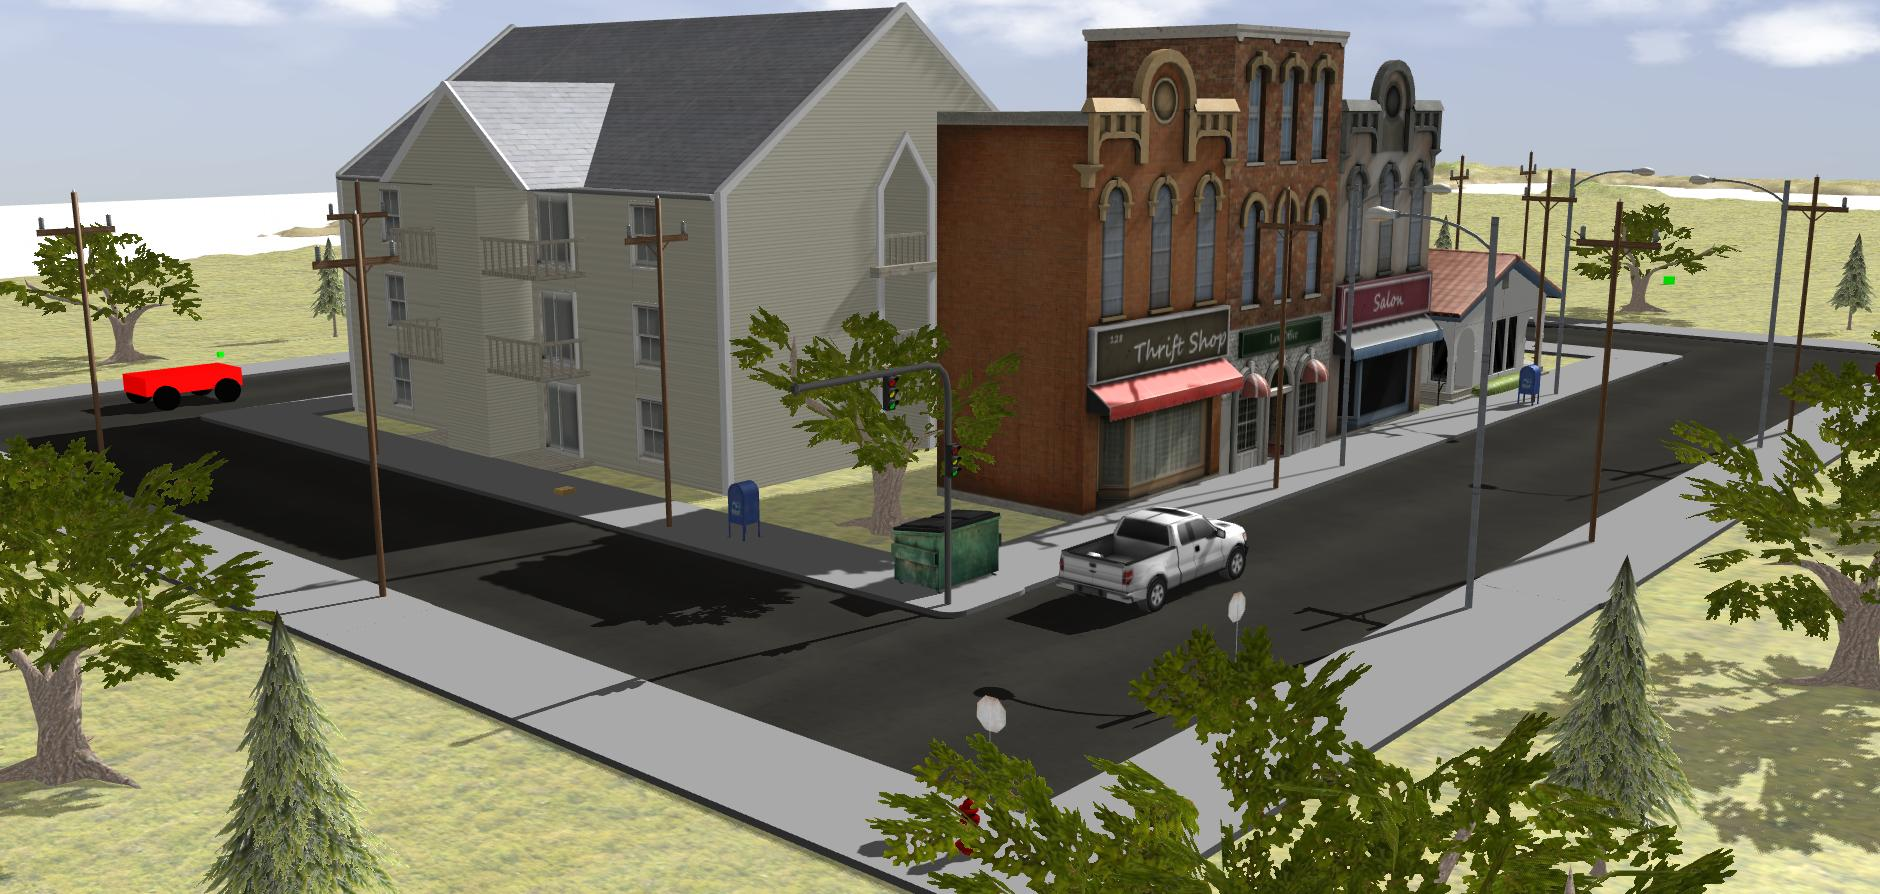
\includegraphics[width=8cm]{figs/simulator}
	\end{center}
	\caption{Modelo de la ciudad original y la ciudad modificada en \textit{Gazebo}.}
	\label{fig:city}
\end{figure}\

El modelo de esta ciudad es estático, es decir, no contiene elementos dinámicos, por lo que es necesario añadir dos tipos de elementos; un semáforo y un peatón que cruce un paso de peatones. Para ello, es necesario añadir dos plugins para \textit{Gazebo}. En primer lugar, y usando un modelo \textit{SDF} que integra el \textit{plugin} de cambio de color en el semáforo\footnote{\url{https://github.com/robustify/gazebo_traffic_light}}. Dicho plugin tiene asociado un fichero de configuración en formato YAML, código  \ref{cod:trafficlight}, en el que se especifica la secuencia de estados del semáforo y su duración en el tiempo.\\

\begin{code}[h]
	\begin{lstlisting}
		light_sequence:
  - { color: "green", duration: 10, flashing: false }
  - { color: "yellow", duration: 1, flashing: false }
  - { color: "red", duration: 50, flashing: false }
	\end{lstlisting}
	\caption[Definición de estados y duraciones del semáforo]{Definición de estados y duraciones del semáforo}
	\label{cod:trafficlight}
\end{code}


El segundo plugin proporciona movimiento a un modelo de un humano llamado actor. Está disponible en otro repositiorio\footnote{\url{https://github.com/BruceChanJianLe/gazebo-plugin-autonomous-actor}} de GitHub y permite que el humano se desplace en el mundo de forma realista. El plugin citado también permite configuración para especificar la ruta de puntos o \textit{waypoints} que el peatón ha de seguir, así como, su velocidad o la distancia mínima a la que debe situarse respecto a un obstáculo. Dicha configuración se realiza directamente en el fichero SDF, como muestra el código \ref{cod:pedestrianconfiguration}.\\

\begin{code}[h]
	\begin{lstlisting}
		<actor name="actor">
			[...]
			<plugin name="trajectory" filename="libTrajectoryActorPlugin.so">
					<target>
					2.4028 -6.9143 1.1 1.570796 -0.0 3.141593
				</target>
					<target>
					2.4028 6.6816 1.1 1.570796 -0.0 3.141593
				</target>
					<velocity>0.75</velocity>
					<obstacle_margin>1.5</obstacle_margin>
					<obstacle></obstacle>
				</plugin>
			</actor>
	\end{lstlisting}
	\caption[Configuración de \textit{waypoints}, velocidad y distancia a obstáculos del peatón]{Configuración de \textit{waypoints}, velocidad y distancia a obstáculos del peatón}
	\label{cod:pedestrianconfiguration}
\end{code}

Ambos modelos se sitúan en una paso de peatones, creado a partir de láminas blancas, produciendo el resultado de la figura \ref{fig:trafficlightpedestrian}.\\

\begin{figure} [h!]
	\begin{center}
		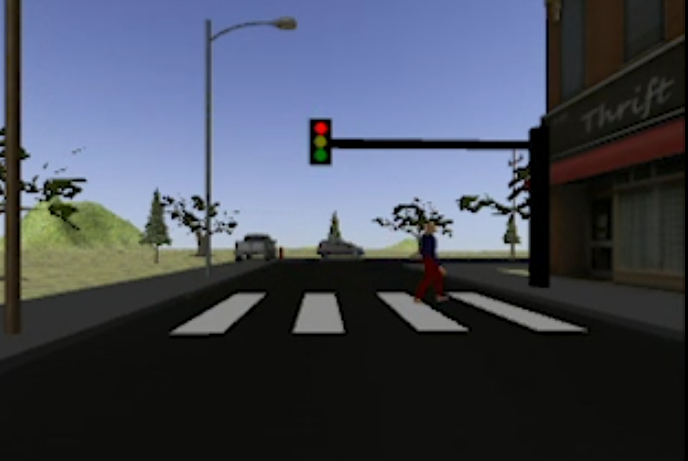
\includegraphics[width=8cm]{figs/trafficlightpedestrian}
	\end{center}
	\caption{Semáforo y peatón usando plugins para \textit{Gazebo}.}
	\label{fig:trafficlightpedestrian}
\end{figure}\


\subsection{Modelo del coche autónomo}
El primer paso para desarrollar un modelo es diseñar las piezas a utilizar, para ello, como se explicó en el capítulo 2, se utilizará \textit{FreeCAD}. El segundo paso es ensamblar el robot con \textit{Blender} utilizando el \textit{add-on} \textit{Phobos} para definir los links y joints del robot con el objetivo de dotar al robot de movimiento, generando un fichero \textit{URDF}. Por último, es necesario modificar el \textit{URDF} para añadir cámaras y controladores para los motores que serán usados en el simulador \textit{Gazebo}.\\

\subsubsection{Diseño de las piezas en \textit{FreeCAD}}

A través de la herramienta \textit{Sketcher}\footnote{\url{https://wiki.freecadweb.org/Sketcher_Workbench}}, disponible en \textit{FreeCAD}, es posible realizar un diseño de piezas en 2D con restricciones de horizontalidad, verticalidad, igualdad entre rectas, medidas, ángulos etc y después convertir dicha pieza en 3D proporcionando un volumen a la pieza. Utilizando dicha herramienta se diseña el chasis y las ruedas del vehículo tomando las medidas reales, lo que da como resultado el diseño de las piezas en 2D de la figura \ref{fig:design2Dfreecad}.\\

\begin{figure} [h!]
	\begin{center}
		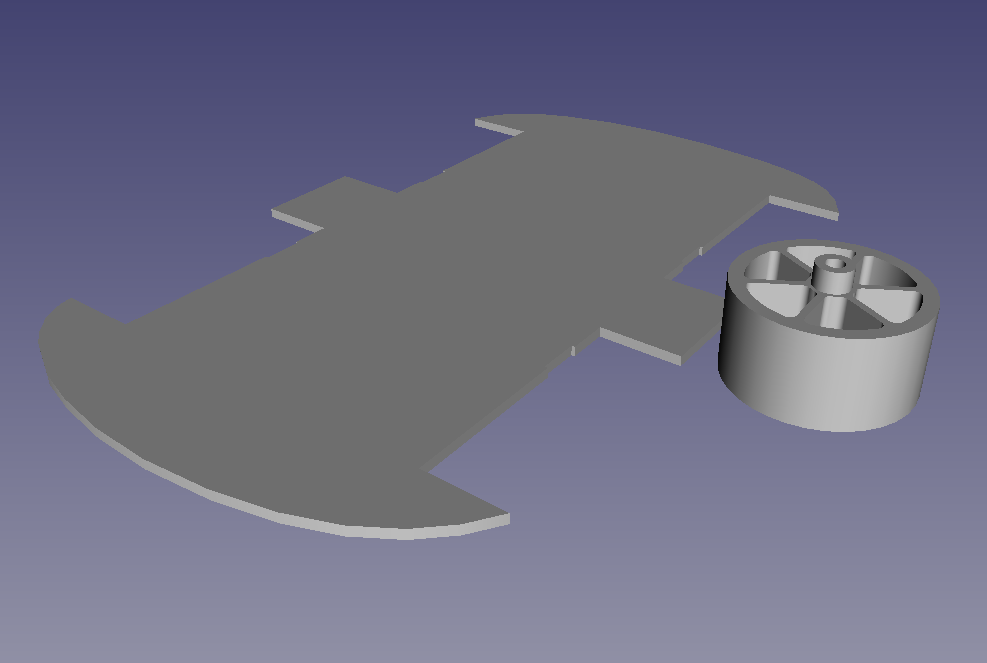
\includegraphics[width=8cm]{figs/freecad}
	\end{center}
	\caption{Diseño de las piezas 2D en \textit{FreeCAD}.}
	\label{fig:design2Dfreecad}
\end{figure}\

A continuación se proporciona una anchura al chasis de 3mm y a las ruedas de xmm, obteniendo el modelo 3D de la figura \ref{fig:design3Dfreecad}.\\

\begin{figure} [h!]
	\begin{center}
		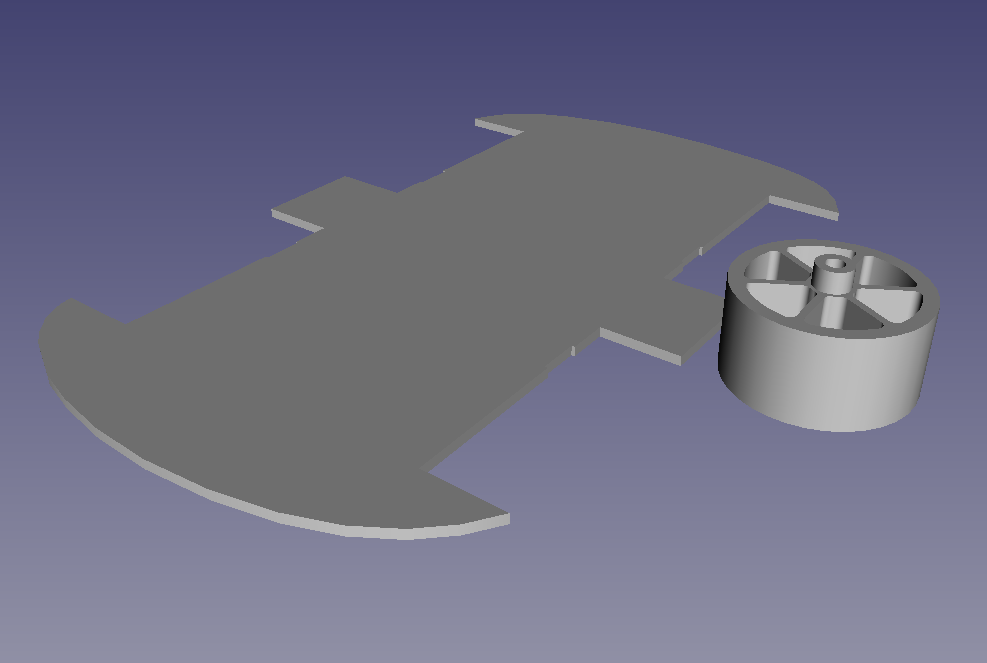
\includegraphics[width=8cm]{figs/freecad}
	\end{center}
	\caption{Diseño de las piezas 3D en \textit{FreeCAD}.}
	\label{fig:design3Dfreecad}
\end{figure}\

El siguiente paso es exportar las piezas diseñadas en formato \textit{STL} para utilizarlas en \textit{Blender}.\\

\subsubsection{Ensamblado del robot en \textit{Blender}}

Una vez importadas las piezas diseñadas en \textit{FreeCAD}, se crean dos unidades del chasis y cuatro ruedas, a continuación se mueven y rotan en el espacio para situarlas correctamente. Con el objetivo de dotar de mayor realismo al modelo, se importan modelos de los motores y la placa utilizados, disponibles en y en. Y se diseñan dos piezas para emular la batería y la cámara del robot. Con todo ello se conforma el modelo estático del robot, figura \ref{fig:blendermodel}.\\

\begin{figure} [h!]
	\begin{center}
		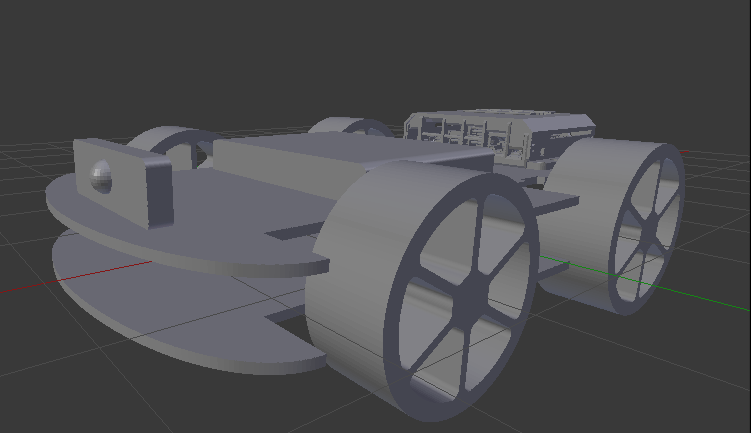
\includegraphics[width=8cm]{figs/blenderModel}
	\end{center}
	\caption{Modelo 3D estático ensamblado en \textit{Blender}.}
	\label{fig:blendermodel}
\end{figure}\

Este modelo es estático, es decir, no es posible simular un movimiento. Para ello es necesario un \textit{add-on} para \textit{Blender} como \textit{Phobos}, que como se explicó anteriormente, permite crear links y \textit{joints} y definir una jerarquía entre ellos.\\

En primer lugar, es necesario definir los elementos visuales que compondrán el modelo, en este caso serán todas las piezas del robot, dichas piezas serán del tipo \textit{mesh}, ya que no son objetos primitivos, como cajas o esferas.\\

A continuación, se define un \textit{link} principal que será el cuerpo delrobot, de este \textit{link} dependerán las cuatro ruedas del vehículo. Con el objetivo de simular colisiones, se crea un modelo de colisión de cada una de
las piezas y un modelo inercial, que estará relacionado con el peso simulado de cada pieza.\\

Por último, se definen los \textit{joints} de cada rueda. A través de está funcionalidad es posible aplicar fuerza o velocidad a las ruedas del robot. Existen diferentes tipos de \textit{joints} en \textit{Phobos}; \textit{fixed}, \textit{revolute}, \textit{continuous}, \textit{prismatic}, en este caso, son necesarios \textit{joints} de tipo \textit{continuous}, ya que las ruedas realizan un giro sin un límite fijado, y no un movimiento transversal.\\

Una vez definidos todos los elementos del modelo y su jerarquía, en el menú lateral de \textit{Blender} se encontrará el diagrama del modelo, figura \ref{fig:blenderdiagram}.\\

\begin{figure} [h!]
	\begin{center}
		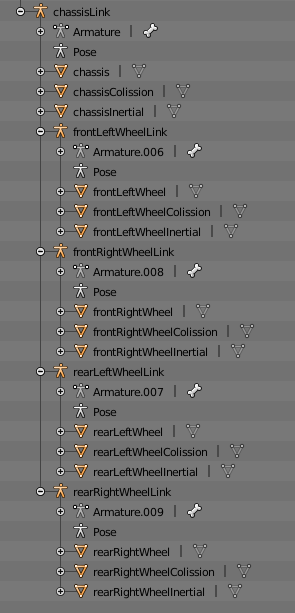
\includegraphics[width=6cm]{figs/phobosDiagram}
	\end{center}
	\caption{Diagrama del modelo diseñado con \textit{Phobos}.}
	\label{fig:blenderdiagram}
\end{figure}\

El siguiente paso es exportar el modelo a formato \textit{URDF}, que como se explicó anteriormente, es el aceptado por \textit{Gazebo} para simular modelos de robots. Las mallas, que componen el modelo visual y de colisiones, se exportan en formato \textit{DAE}, y se cargan desde el modelo \textit{URDF}.\\


\subsubsection{Adición de plugins para Gazebo}

Con el objetivo de mover el robot utilizando el middleware ROS, es necesario cargar el plugin \textit{Gazebo ROS Control} mediante el código \ref{cod:gazeboroscontrol}.\\

\begin{code}[h]
	\begin{lstlisting}[language=XML]
		<gazebo>
		<plugin name="gazebo_ros_control" filename="libgazebo_ros_control.so">
			<robotNamespace>/autonomous_vehicle</robotNamespace>
		</plugin>
		</gazebo>
	\end{lstlisting}
	\caption[Código para cargar el plugin \textit{Gazebo ROS Control}]{Código para cargar el plugin \textit{Gazebo ROS Control}}
	\label{cod:gazeboroscontrol}
\end{code}

Otro elemento a añadir en el fichero URDF, es la existencia de dos cámaras; una cámara onboard y otra situada encima del robot que proporcionará una visión de la ruta realizada. Dichas cámaras simuladas publicarán su imagen en un topic de ROS con una resolución y un formato fijado meidante el código \ref{cod:gazebocamera}.\\

\begin{code}[h]
	\begin{lstlisting}[language=XML]
	<gazebo reference="onboardCameraLink">
		<sensor name='cam_sensor' type='camera'>
			[...]
			<camera name='onboardCameraLink'>
				<horizontal_fov>1.570000</horizontal_fov>
				<image>
					<width>320</width>
					<height>240</height>
					<format>R8G8B8</format>
				</image>
				[...]
			</camera>
			[...]
		</sensor>
	</gazebo>
	\end{lstlisting}
	\caption[Código para crear cámara simulada en \textit{Gazebo}]{Código para crear cámara simulada en \textit{Gazebo}}
	\label{cod:gazebocamera}
\end{code}

Para mover el robot simulado también será necesario un fichero \textit{YAML}, en el que se especifiquen los controladores de los \textit{joints} y el nombre de los \textit{topics} en los que se publicarán los mensajes mendiante el código \ref{cod:controllers}.\\

\begin{code}[h]
	\begin{lstlisting}
		autonomous_vehicle:
		joint_state_controller:
			type: joint_state_controller/JointStateController
			publish_rate: 10
		front_right_wheel_velocity_controller:
			type: velocity_controllers/JointVelocityController
			joint: frontRightWheelJoint
		front_left_wheel_velocity_controller:
			type: velocity_controllers/JointVelocityController
			joint: frontLeftWheelJoint
		rear_right_wheel_velocity_controller:
			type: velocity_controllers/JointVelocityController
			joint: rearRightWheelJoint
		rear_left_wheel_velocity_controller:
			type: velocity_controllers/JointVelocityController
			joint: rearLeftWheelJoint
	\end{lstlisting}
	\caption[Definición de los controladores de los \textit{joints} del robot]{Definición de los controladores de los \textit{joints} del robot}
	\label{cod:controllers}
\end{code}

Con todo ello, se implementa un \textit{launcher} \footnote{\url{https://github.com/jmvega/tfg-amariscal/src/launcher......}} que lanza el modelo dińamico del robot y se muestra en la ciudad simulada, figura \ref{fig:modelGazebo}.

\begin{figure} [h!]
	\begin{center}
		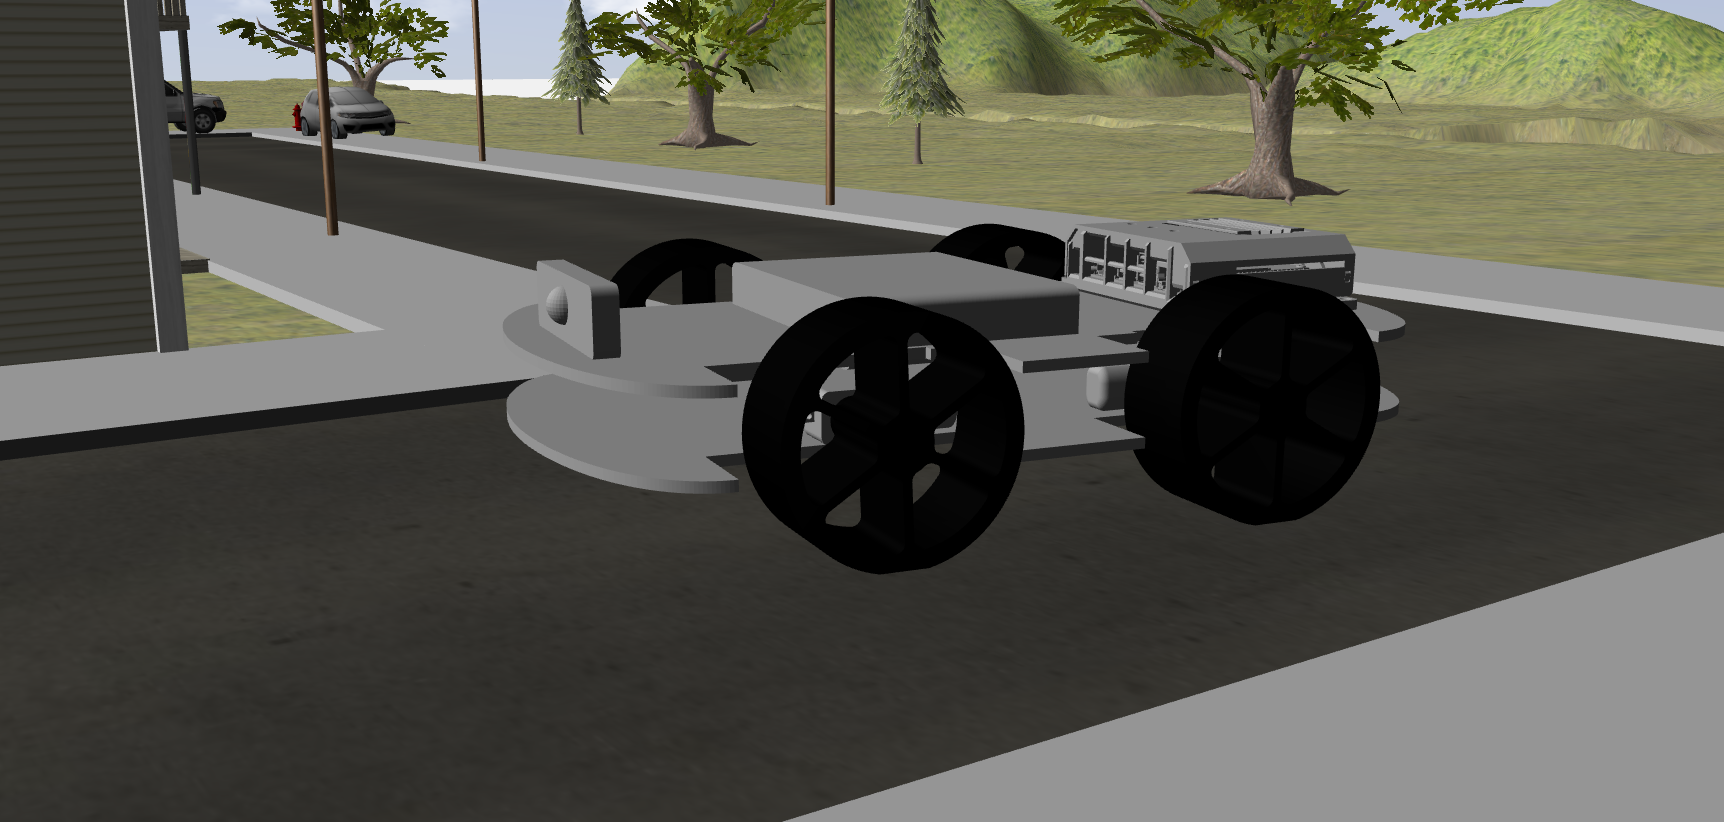
\includegraphics[width=12cm]{figs/modelGazebo}
	\end{center}
	\caption{Modelo dinámico del robot en \textit{Gazebo}.}
	\label{fig:modelGazebo}
\end{figure}\

\subsection{Seguimiento de carril}

\subsection{Detección de objetos}

\section{Entorno real}

\section{Snippets}

Puede resultar interesante, para clarificar la descripción, mostrar fragmentos de código (o \textit{snippets}) ilustrativos. En el Código \ref{cod:codejemplo} vemos un ejemplo escrito en \texttt{C++}.

\begin{code}[h]
	\begin{lstlisting}[language=C++]
void Memory::hypothesizeParallelograms () {
  for(it1 = this->controller->segmentMemory.begin(); it1++) {
    squareFound = false; it2 = it1; it2++;
    while ((it2 != this->controller->segmentMemory.end()) && (!squareFound)) {
      if (geometry::haveACommonVertex((*it1),(*it2),&square)) {
        dist1 = geometry::distanceBetweenPoints3D ((*it1).start, (*it1).end);
        dist2 = geometry::distanceBetweenPoints3D ((*it2).start, (*it2).end);
      }
    // [...]
\end{lstlisting}
	\caption[Función para buscar elementos 3D en la imagen]{Función para
		buscar elementos 3D en la imagen}
	\label{cod:codejemplo}
\end{code}

En el Código \ref{cod:codejemplo2} vemos un ejemplo escrito en \texttt{Python}.

\begin{code}[h]
	\begin{lstlisting}[language=Python]
def mostrarValores():
    print (w1.get(), w2.get())

master = Tk()
w1 = Scale(master, from_=0, to=42)
w1.pack()
w2 = Scale(master, from_=0, to=200, orient=HORIZONTAL)
w2.pack()
Button(master, text='Show', command=mostrarValores).pack()

mainloop()
\end{lstlisting}
	\caption[Cómo usar un Slider]{Cómo usar un Slider}
	\label{cod:codejemplo2}
\end{code}

\section{Verbatim}

Para mencionar identificadores usados en el código ---como nombres de funciones
o variables--- en el texto, usa el entorno literal o verbatim
\verb|hypothesizeParallelograms()|. También se puede usar este entorno para varias líneas,
como se ve a continuación:

\begin{verbatim}
void Memory::hypothesizeParallelograms () {
  // add your code here
}
\end{verbatim}

\section{Ecuaciones}

Si necesitas insertar alguna ecuación, puedes hacerlo. Al igual que las
figuras, no te olvides de referenciarlas. A continuación se exponen algunas
ecuaciones de ejemplo: Ecuación \ref{ec:ec1} y Ecuación \ref{ec:ec2}.

\begin{myequation}[h]
	\begin{equation}
		H = 1 - \frac{\sum_{i=0}^{N}\frac{(\frac{d_{j_s} +
					d_{j_e}}{2})}{N}}{M}
		\nonumber
		\label{ec:ec1}
	\end{equation}
	\caption[Ejemplo de ecuación con fracciones]{Ejemplo de ecuación con
		fracciones}
\end{myequation}

\begin{myequation}[h]
	\begin{equation}
		v(entrada)= \left\{
		\begin{array}{lcc}
			0                   & \mbox{if} & \epsilon_t < 0.1
			\\
			K_p\cdot{(T_{t}-T)} & \mbox{if} & 0.1 \leq \epsilon_t <
			M_t
			\\
			K_p \cdot M_t       & \mbox{if} & M_t < \epsilon_t
		\end{array}
		\right.
		\label{ec:ec2}
	\end{equation}
	\caption[Ejemplo de ecuación con array y letras y símbolos
		especiales]{Ejemplo de ecuación con array y letras y símbolos
		especiales}
\end{myequation}

\section{Tablas o cuadros}

Si necesitas insertar una tabla, hazlo dígnamente usando las propias tablas de
\LaTeX, no usando pantallazos e insertándolas como figuras... En el Cuadro
\ref{cuadro:ejemplo} vemos un ejemplo.

\begin{table}[H]
	\begin{center}
		\begin{tabular}{|c|c|}
			\hline
			\textbf{Parámetros}   & \textbf{Valores}
			\\
			\hline
			Tipo de sensor        & Sony IMX219PQ[7] CMOS 8-Mpx
			\\
			Tamaño del sensor     & 3.674 x 2.760 mm (1/4" format)
			\\
			Número de pixels      & 3280 x 2464 (active pixels)
			\\
			Tamaño de pixel       & 1.12 x 1.12 um
			\\
			Lente                 & f=3.04 mm, f/2.0
			\\
			Ángulo de visión      & 62.2 x 48.8 degrees
			\\
			Lente SLR equivalente & 29 mm
			\\
			\hline
		\end{tabular}
		\caption{Parámetros intrínsecos de la cámara}
		\label{cuadro:ejemplo}
	\end{center}
\end{table}


Language YAML, XML?